% Options for packages loaded elsewhere
\PassOptionsToPackage{unicode}{hyperref}
\PassOptionsToPackage{hyphens}{url}
%
\documentclass[
]{article}
\usepackage{amsmath,amssymb}
\usepackage{lmodern}
\usepackage{iftex}
\ifPDFTeX
  \usepackage[T1]{fontenc}
  \usepackage[utf8]{inputenc}
  \usepackage{textcomp} % provide euro and other symbols
\else % if luatex or xetex
  \usepackage{unicode-math}
  \defaultfontfeatures{Scale=MatchLowercase}
  \defaultfontfeatures[\rmfamily]{Ligatures=TeX,Scale=1}
\fi
% Use upquote if available, for straight quotes in verbatim environments
\IfFileExists{upquote.sty}{\usepackage{upquote}}{}
\IfFileExists{microtype.sty}{% use microtype if available
  \usepackage[]{microtype}
  \UseMicrotypeSet[protrusion]{basicmath} % disable protrusion for tt fonts
}{}
\makeatletter
\@ifundefined{KOMAClassName}{% if non-KOMA class
  \IfFileExists{parskip.sty}{%
    \usepackage{parskip}
  }{% else
    \setlength{\parindent}{0pt}
    \setlength{\parskip}{6pt plus 2pt minus 1pt}}
}{% if KOMA class
  \KOMAoptions{parskip=half}}
\makeatother
\usepackage{xcolor}
\usepackage[margin=1in]{geometry}
\usepackage{graphicx}
\makeatletter
\def\maxwidth{\ifdim\Gin@nat@width>\linewidth\linewidth\else\Gin@nat@width\fi}
\def\maxheight{\ifdim\Gin@nat@height>\textheight\textheight\else\Gin@nat@height\fi}
\makeatother
% Scale images if necessary, so that they will not overflow the page
% margins by default, and it is still possible to overwrite the defaults
% using explicit options in \includegraphics[width, height, ...]{}
\setkeys{Gin}{width=\maxwidth,height=\maxheight,keepaspectratio}
% Set default figure placement to htbp
\makeatletter
\def\fps@figure{htbp}
\makeatother
\setlength{\emergencystretch}{3em} % prevent overfull lines
\providecommand{\tightlist}{%
  \setlength{\itemsep}{0pt}\setlength{\parskip}{0pt}}
\setcounter{secnumdepth}{-\maxdimen} % remove section numbering
\ifLuaTeX
  \usepackage{selnolig}  % disable illegal ligatures
\fi
\IfFileExists{bookmark.sty}{\usepackage{bookmark}}{\usepackage{hyperref}}
\IfFileExists{xurl.sty}{\usepackage{xurl}}{} % add URL line breaks if available
\urlstyle{same} % disable monospaced font for URLs
\hypersetup{
  pdftitle={Tarea Empírica 1 - Macroeconometría},
  pdfauthor={Profesor: Mauricio Tejada - Estudiante: Matías Vicuña},
  hidelinks,
  pdfcreator={LaTeX via pandoc}}

\title{Tarea Empírica 1 - Macroeconometría}
\author{Profesor: Mauricio Tejada - Estudiante: Matías Vicuña}
\date{16/08/2022}

\begin{document}
\maketitle

\hypertarget{desarrollo}{%
\subsection{Desarrollo}\label{desarrollo}}

Para comenzar, desarrollamos a partir de la data
\emph{``datos\_ejercicio\_empirico\_1.xlsx''} entregados las siguientes
gráficas:

1- Comenzamos con la gráfica de precios históricos de la bencina desde
1985 hasta 2022, añadimos además que esta gráfica contiene los precios
\textbf{\emph{Linealizados}}, por lo que se le ha aplicado \(ln()\).

\hypertarget{gruxe1fico-1.1}{%
\subsubsection{Gráfico 1.1}\label{gruxe1fico-1.1}}

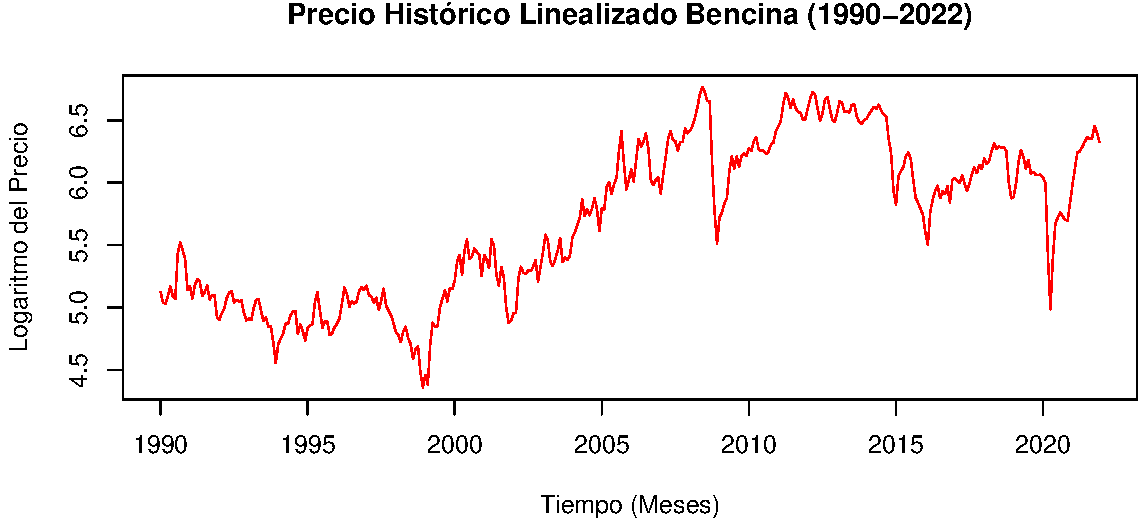
\includegraphics{Tarea-1---Matías-Vicuña_files/figure-latex/plot-bencina-1.pdf}

Con este gráfico vemos que el precio de la bencina estos últimos años a
tenido una tendencia alzista, viendo un incremento notorio desde finales
de los '90 hasta comienzo del 2010, luego de ello, se ha visto que el
precio de la bencina ha tomado una paridad, manteniendo una varianza
bastante pareja por 10 años, hasta la llegada del 2020 dónde el impacto
de la crisis sanitaria global impactó notoriamente esta constancia de
precios.

Ahora bien, en el caso de los precios históricos del petróleo en los
mismos años se ve una semejanza en cuanto a volatilidad, varianza y
fechas clave de alteración de los precios, esto da un primer vistazo a
lo que en la parte 2 analizaré mas en detalle, denotando así la gran
correlación que ambos bienes tienen.

\newpage

Siguendo el análisis anterior, en el siguiente gráfico vemos los precios
del petróleo \textbf{\emph{Linealizados}}, por lo cual se observara que
los datos en si son mas pequeños de lo que se aprecia en el Excel.

\hypertarget{gruxe1fico-2.1}{%
\subsubsection{Gráfico 2.1}\label{gruxe1fico-2.1}}

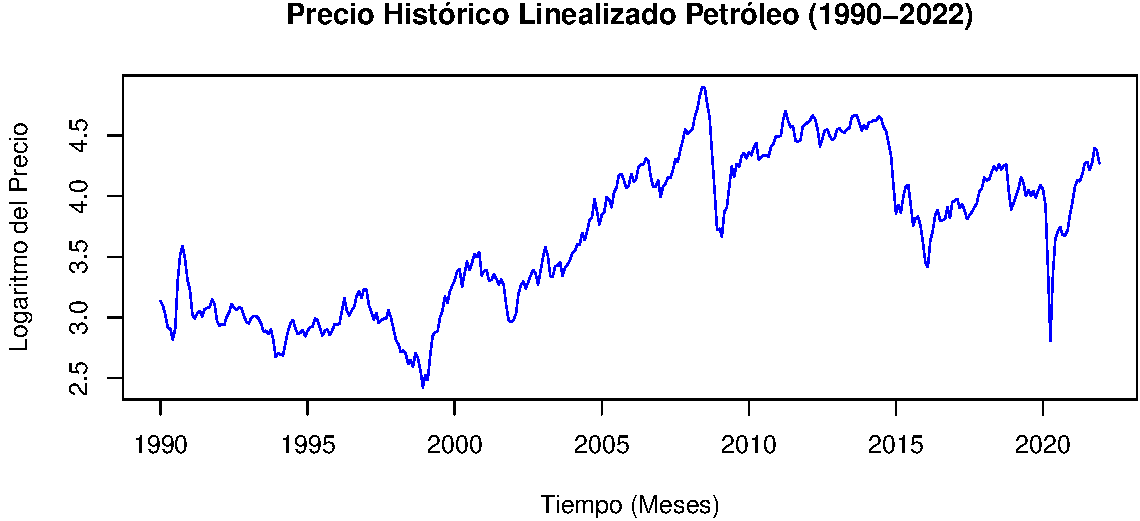
\includegraphics{Tarea-1---Matías-Vicuña_files/figure-latex/plot petroleo-1.pdf}

Analizando el gráfico vemos (al igual que en el gráfico 1) una tendencia
entre finales de los '80s y comienzo de los '00s constante, manteniendo
un promedio bastante lineal y una varianza similar en el tiempo, ahora,
desde el 2000 hasta principios del 2010 se ve una tendencia positiva del
incremento del precio. Además de ello, y al igual que en el gráfico 1,
se ve entre 2010 y finales de la década una tendencia promedio bastante
lineal, conservando esta dinámica hasta fines del 2019, dónde los
efectos COVID distorcionó este movimiento.

\newpage

2- Ahora, visualizaremos como se comportan cada una de las varibles
graficamente realizando una autocorrelación con 10 Regazos, con ello
observaremos cuan relacionados son en el tiempo los precios de cada uno
de los bienes.

Comenzaremos viendo la gráfica del precio del petróleo linealizado en el
mismo tramo temporal que en la pregunta 1 (1985-2022).

\hypertarget{gruxe1fica-1.2}{%
\subsubsection{Gráfica 1.2}\label{gruxe1fica-1.2}}

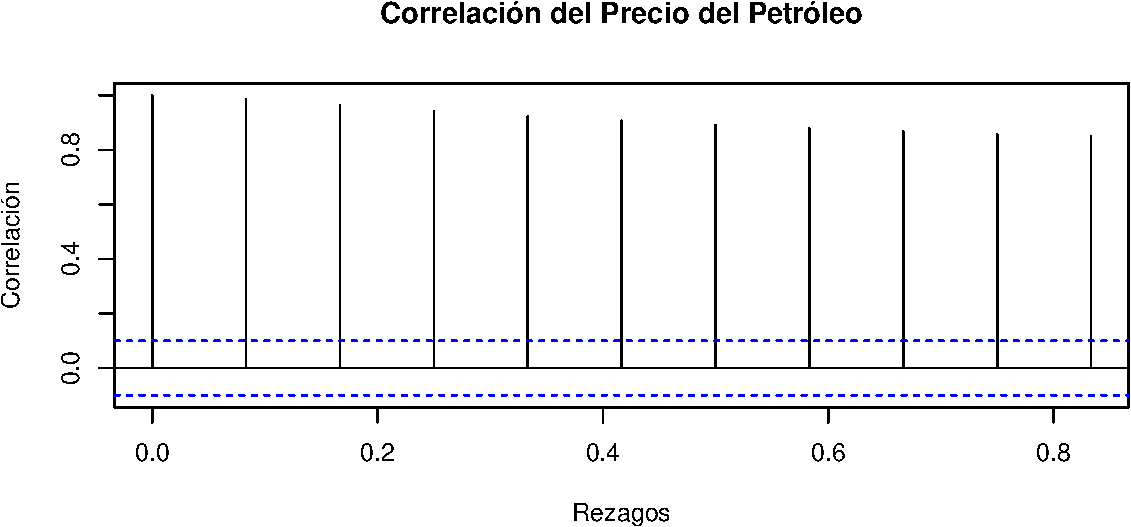
\includegraphics{Tarea-1---Matías-Vicuña_files/figure-latex/plot autocorrelacion petroleo-1.pdf}

Se puede observar en la gráfica 1.2 el como en el tiempo la correlación
que tiene el precio con el precio pasado del petróleo mantiene una
correlación cercana a 1, por lo que podemos concluir que el precio del
mismo tiene una alta dependencia de su mismo pasado para el precio
futuro.

Ahora observaremos también la gráfica de autocorrelación pero del precio
de la bencina, con ella obtendremos conclusiones muy similares a la
gráfica anterior.

\hypertarget{gruxe1fica-2.2}{%
\subsubsection{Gráfica 2.2}\label{gruxe1fica-2.2}}

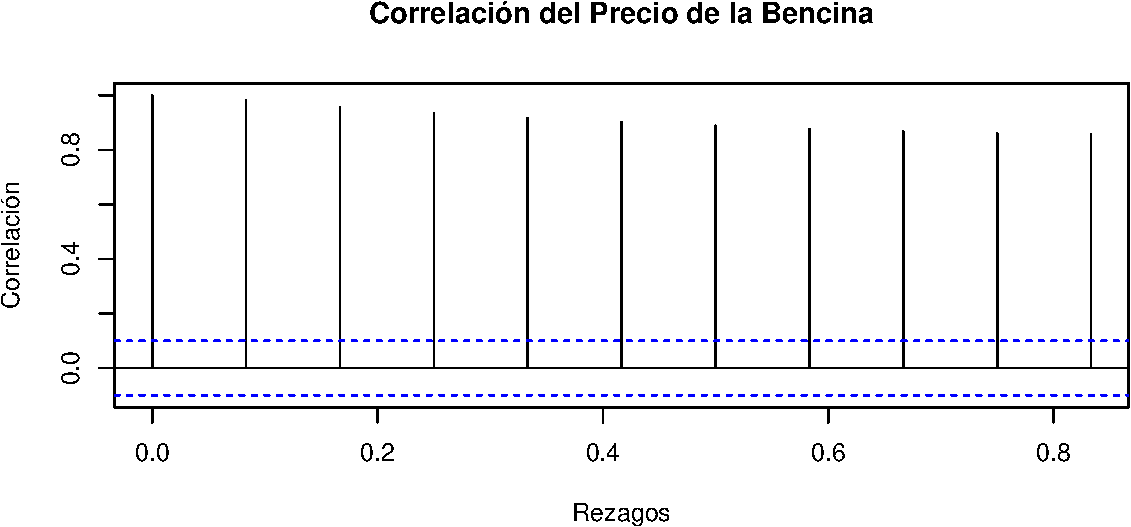
\includegraphics{Tarea-1---Matías-Vicuña_files/figure-latex/plot autocorrelacion Bencina-1.pdf}

\newpage

Continuando al gráfico anterior, se logra ver los precios pasado de la
bencina tiene una directa relación sobre el precio del futuro del mismo,
esto ya que se ve con 10 de rezasgo, que la autocorrelación hasta el
último periodo de rezago sigue siendo mayor o igual a 0.8.

3- Transformando nuestra data con la primera diferencia, podremos
apreciar un efecto de ``ruido'' en las series de tiempo particulares,
comenzaremos visualizando la primera diferencia del logaritmo natural
del petróleo:

\hypertarget{gruxe1fico-1.3}{%
\subsubsection{Gráfico 1.3}\label{gruxe1fico-1.3}}

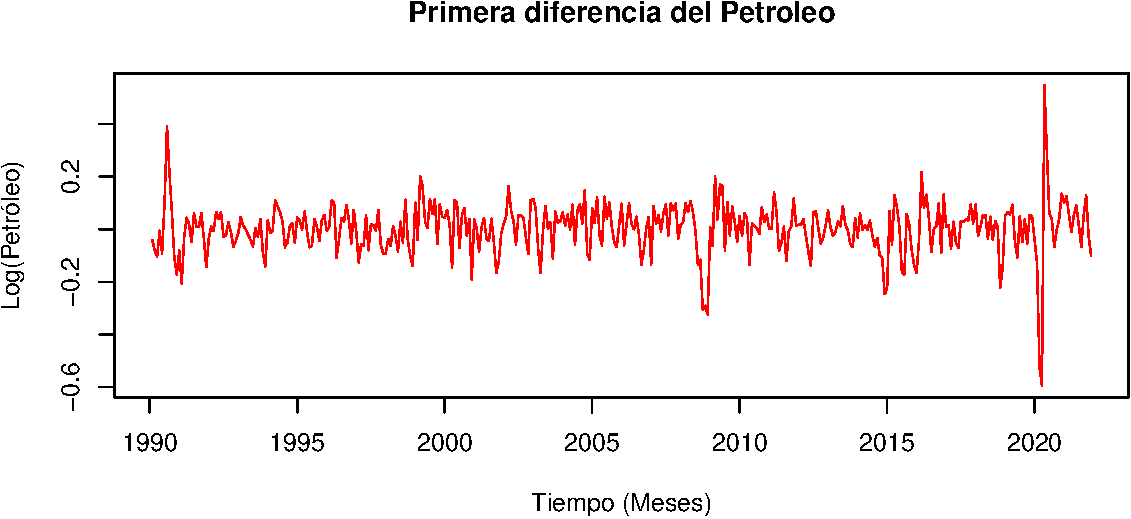
\includegraphics{Tarea-1---Matías-Vicuña_files/figure-latex/plot diff petroleo-1.pdf}

Se logra observar que la serie de tiempo posee una estructura con media
bastante constante, una varianza del mismo modo semejante en ``casi''
todos los periodos, es por eso que se aprecia que las variaciones
(descontando la tendencia) son en cierta forma con una estructura
estacionaria de la misma forma en todos los periodos.

\hypertarget{gruxe1fico-2.3}{%
\subsubsection{Gráfico 2.3}\label{gruxe1fico-2.3}}

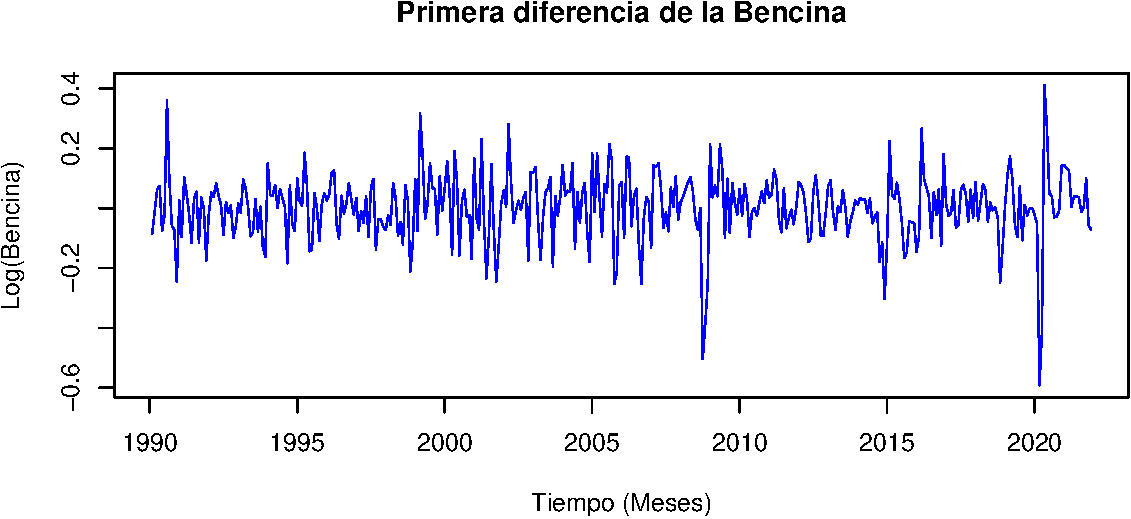
\includegraphics{Tarea-1---Matías-Vicuña_files/figure-latex/plot diff bencina-1.pdf}

Al igual que en gráfico anterior, se ve un ajuste de la varianza por la
estacionariedad de la muestra, por lo que se denota visiblemente que la
media y la varianza se comportan de manera ciertamente constante.

\newpage

4- Ahora, considerando las primeras diferencias de ambos bienes, se
visualizará la autocorrelación de las primeras diferencias, apreciando
un cambio notorio en la correlación de periodos anteriores, para ello,
se considerará un límite de 10 rezagos por cada autocorrelación.

\hypertarget{gruxe1fica-1.4}{%
\subsubsection{Gráfica 1.4}\label{gruxe1fica-1.4}}

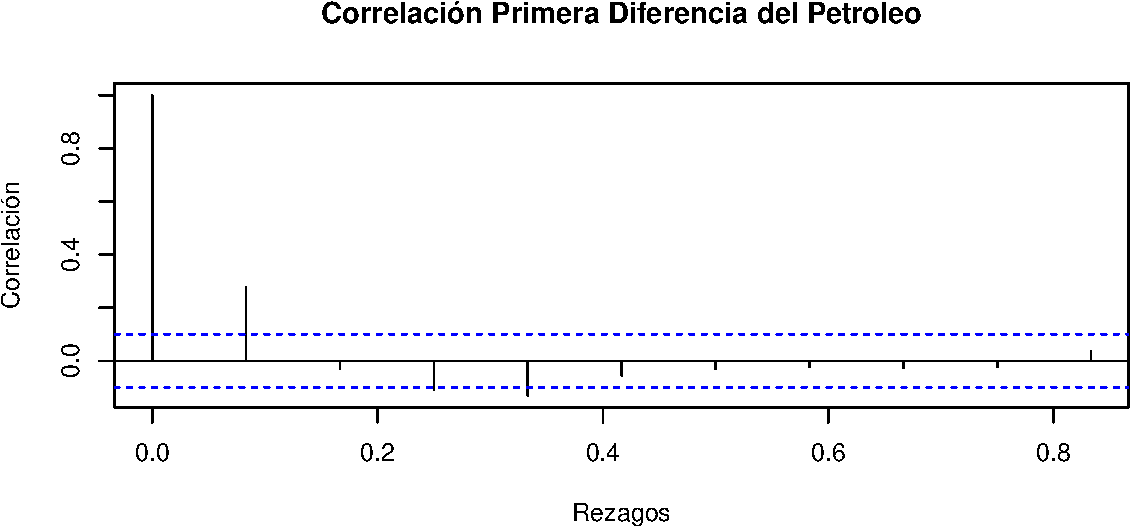
\includegraphics{Tarea-1---Matías-Vicuña_files/figure-latex/plot autocorrelación diff petroleo-1.pdf}

En esa gráfica de autocorrelación se percibe un gran cambio sobre la
misma gráfica del punto 1.2, ahora, desde el primer periodo de rezago en
adelante, se nota como la correlación en el precio del presente sobre el
precio pasado es casi nula, desde la segunda ya se denota una
correlación negativa.

\hypertarget{gruxe1fica-2.4}{%
\subsubsection{Gráfica 2.4}\label{gruxe1fica-2.4}}

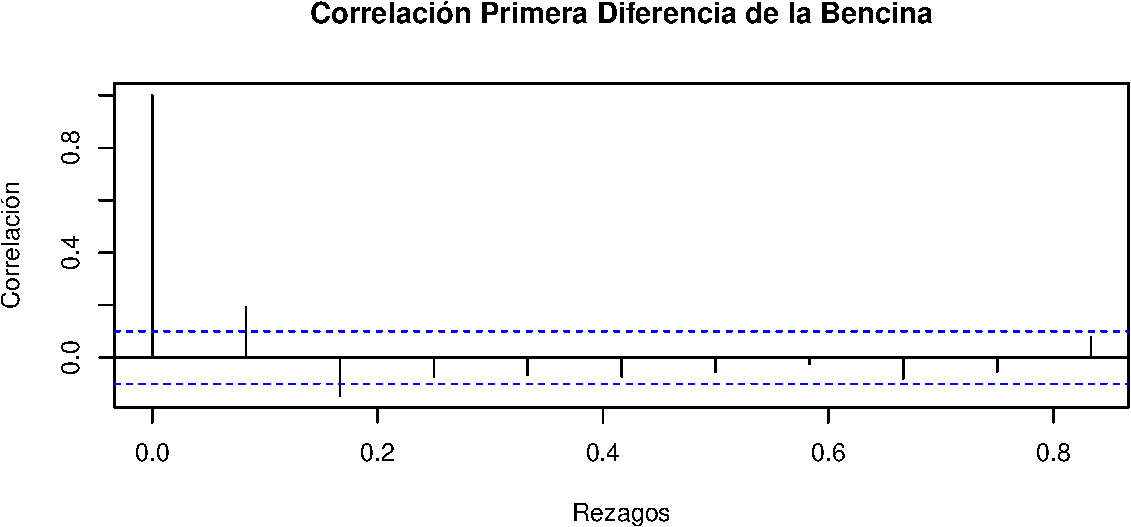
\includegraphics{Tarea-1---Matías-Vicuña_files/figure-latex/plot autocorrelación diff bencina-1.pdf}

Al igual que en el gráfico anterior, se ve como la correlación por cada
rezago posterior va disminuyendo llegando a puntos negativos, es decir
que, el precio futuro de la bencina no tiene relación o influencias por
el precio pasado del mismo.

\newpage

5- Luego de todo el análisis anterior hecho de la data, se mostrará de
manera gráfica en formato anual las mismas gráficas presentadas en el
punto 1.1 y 1.2, pero con una diferencia notoría de suavización de las
líneas dado que se agrupan los datos en formato anual.

\hypertarget{gruxe1fico-1.5}{%
\subsubsection{Gráfico 1.5}\label{gruxe1fico-1.5}}

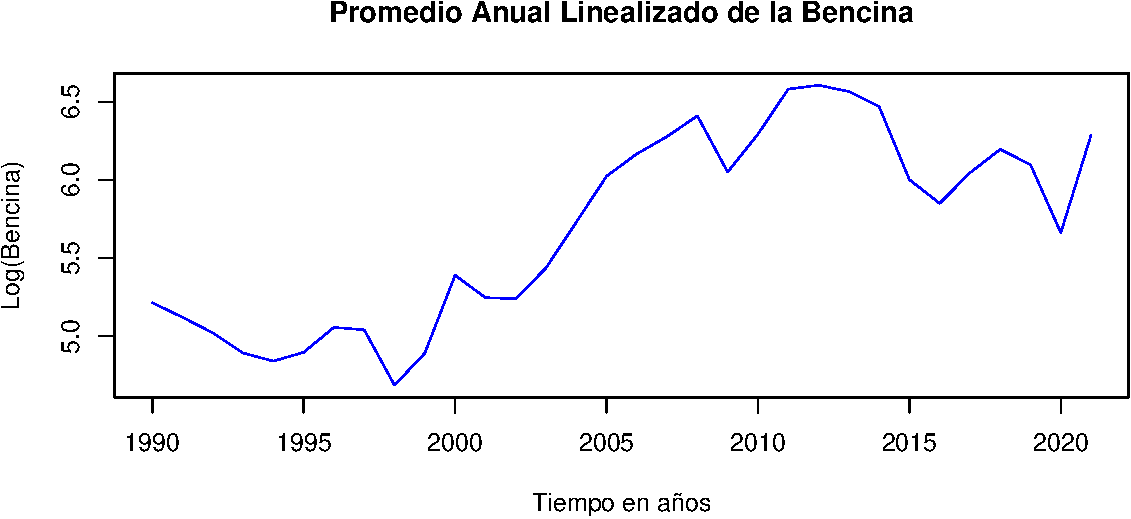
\includegraphics{Tarea-1---Matías-Vicuña_files/figure-latex/ploteo anual bencina-1.pdf}

\vspace{3mm}

\hypertarget{gruxe1fica-2.5}{%
\subsubsection{Gráfica 2.5}\label{gruxe1fica-2.5}}

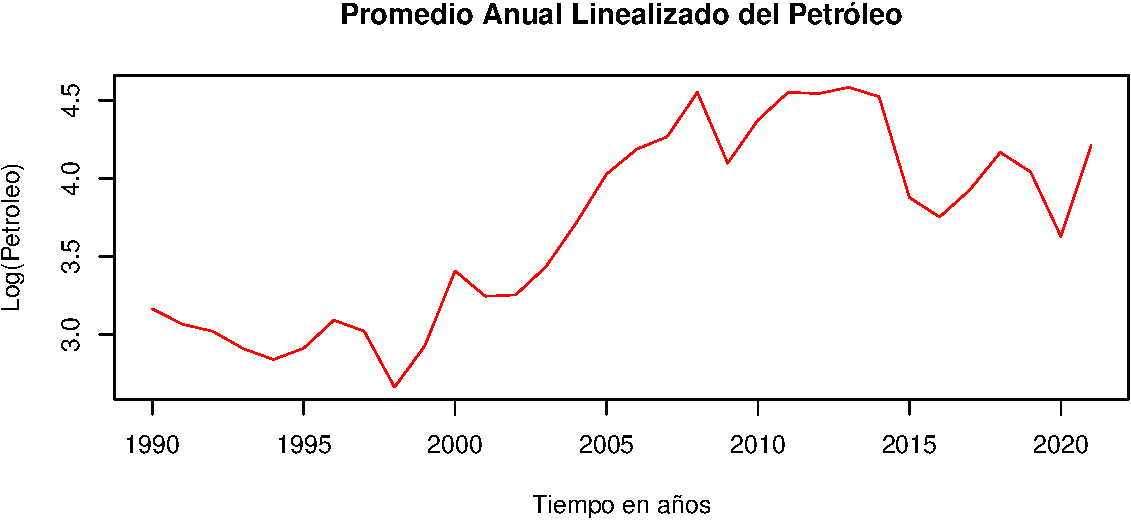
\includegraphics{Tarea-1---Matías-Vicuña_files/figure-latex/ploteo anual petroleo-1.pdf}

\end{document}
